\documentclass[a4paper, norsk, 12pt]{article}
\usepackage[T1]{fontenc}
\usepackage{fancyvrb}
%\documentclass{article} % was article, thought i'd try with report...
\usepackage{float}
%\usepackage{fullpage} % 1 inch margins
%\usepackage{harvard} % harvard reference style++
\usepackage[hidelinks]{hyperref} % do not remember entirely what this does
%%\usepackage{minted} % [LINUXONLY] list environment with code highlighting
\usepackage[utf8]{inputenc} %To get æøå
\usepackage[norsk]{babel} %Does it norway'ish
%\setcounter{chapter}{-1} %chapter numeration to start on 0
%\usepackage{titlesec} %To make chapter headings different
\usepackage[margin=2.5cm]{geometry}
%\usepackage{longtable} %Table that breakes pages
%\usepackage{tabularx} %Table that breakes lines
\usepackage{ltablex} %Table that combines longtable and tubularx. (Use \begin{tabularx}
\usepackage{graphicx} %To insert image
\usepackage{parskip} %Removes indent and make space between the part sections, like \medskip.
\usepackage[labelformat=empty]{caption} %Removes "Figur 'nr'" in \caption on images.
%\usepackage{color, colortbl} %To use colors in tabulars


\newcommand{\tab}{\hspace*{2em}}

%Removes the indent:
%\setlength\parindent{0pt}

%Changing the paragraph title look:
\makeatletter
\renewcommand\paragraph{\@startsection{paragraph}{4}{\z@}%
  {-3.25ex\@plus -1ex \@minus -.2ex} %To get new line after title
  {1.5ex \@plus .2ex}%
  {\normalfont\large\bfseries}}
\makeatother

%\titleformat{\chapter}[hang]{\bf\huge}{\thechapter}{2pc}{} %To make chapters nice
\title{Oblig 2 \\ IMT3441 \\ Database- og applikasjonsdrift}
\author{Solveig Sørheim 090880 \\ Martin Kristian Mellum 100874}
\date{\today}

%%Useful:
%\hspace*{\fill} \\[-\dimexpr\baselineskip+\parskip\relax] - removes big space after \begin{verbatim}
%\verb - Small kode inline 
%\textt - For bigger kode inline (line breaking)

\begin{document}
\begin{figure}[h!]
 \centering
  
\includegraphics[width=0.5\textwidth]{Images/hig_logo.png}
 %\caption{Bare noko eg skribla på Paint..}
 \maketitle       % make title
\end{figure}
\pagebreak
%%\section{Abstract} % not sure if needed
%%This section is to be written when all else is done. 100-200 words summarizing.
\tableofcontents % make table of contents
\pagebreak	% and break the page, because pretty


\section{Ukesoppgaver Nr. 5 - 15. Februar}
\subsection{Oppgave 1}
På forelesingen den 17. Februar satte Sørheim opp database på db2 som vist i foilerne.

\subsection{Oppgave 2}
På forelesingen den 17. Februar satte Sørheim opp munin-plugin på db2 som vist i foilerne. Senere satte vi opp munin-plugin på db1 som vist i foilerne.

\subsection{Oppgave 3}
I /etc/mysql/my.cnf i db1 og db2 fann vi linjen som inneheldt
\begin{verbatim}
#log_bin
\end{verbatim}
Vi tok bort kommenteringen, slik at binary logging vart enabled.

Deretter restartet vi mysql ved å bruke /etc/init.d/mysql restart
\subsection{Oppgave 4}
I /etc/mysql/my.cnf i db1 og db2 fann vi linjene som assosierte med slow queries og endret de til:
\begin{verbatim}
log_slow_queries        = /var/log/mysql/mysql-slow.log
long_query_time = 5
\end{verbatim}
Deretter tok vi restart på mysql ved koden /etc/init.d/mysql/restart
\subsection{Oppgave 5}
Vi logget oss på mysql databasen bf på db1 fra www1:
\begin{verbatim}
root@www1:~# mysql -h db1 -u bfuser -p bf
Enter password:
\end{verbatim}
Herfra skrev og fikk følgende:
\begin{verbatim}
mysql> show tables;
+--------------+
| Tables_in_bf |
+--------------+
| comments     |
| posts        |
| user         |
+--------------+
3 rows in set (0.00 sec)
mysql> select * FROM user;
Empty set (0.00 sec)
\end{verbatim}
Her ser vi at det ikke er noen brukere ennå.

Vi slet veldig med å finne ut hvordan vi kunne logge oss på databasen bf fjernt. Då vi fann ut hvordan dette skjedde slet vi med å få spørringen til å skje. Den første suksessfulle koden vår var: \hspace*{\fill} \\[-\dimexpr\baselineskip+\parskip\relax]
\begin{verbatim}
mysql -h db1 -u bfuser -pmybfpassword bf -e "show tables;"  
\end{verbatim}
Denne viste oss at vi klarte å kjøre en spørring på databasen.

Vi prøvde oss frem og kom frem til at denne koden virket bra:\hspace*{\fill} \\[-\dimexpr\baselineskip+\parskip\relax]
\begin{verbatim}
mysql -h db1 -u bfuser -pmybfpassword bf -e "select * from user;"
\end{verbatim}
Problemet med den var at den viste navnene og all annen informasjon om brukerne, og vi var bare interessert i antall brukere. Dermed kom vi frem til denne koden:\hspace*{\fill} \\[-\dimexpr\baselineskip+\parskip\relax]
\begin{verbatim}
mysql -h db1 -u bfuser -pmybfpassword bf -e "select COUNT(*) from user;"
\end{verbatim}
Vi prøvde mye med å finne ut hvordan vi kunne lage et perl script for å kjøre bash kommandoer, men la prosjektet på is.

Etter å ha sett på tidligere pdf-er om perl på fronter, fant vi ut at vi kunne bruke “print”  for å kjøre bash kommandoer i perl. Koden så slik ut:\hspace*{\fill} \\[-\dimexpr\baselineskip+\parskip\relax]
\begin{verbatim}
print `mysql -h db1 -u bfuser -pmybfpassword bf -e "select COUNT(*) from user;"`;
\end{verbatim}

\subsection{Oppgave 6}
For å finne ut hvilke tabeller som låg i databasen brukte vi denne kommandoen: \hspace*{\fill} \\[-\dimexpr\baselineskip+\parskip\relax]
\begin{verbatim}
mysql -h db1 -u bfuser -pmybfpassword bf -e "show tables;"
\end{verbatim}

Vi fikk dette resultatet:
\begin{verbatim}
+--------------+
| Tables_in_bf |
+--------------+
| comments     |
| posts        |
| user         |
+--------------+
\end{verbatim}
For å se hvilke enheter som låg under tabellen posts skrev  vi denne spørringen: \hspace*{\fill} \\[-\dimexpr\baselineskip+\parskip\relax]
\begin{verbatim}
mysql -h db1 -u bfuser -pmybfpassword bf -e "select *, COUNT(*) from posts;"
\end{verbatim}
Dermed lagde vi spørringen:\hspace*{\fill} \\[-\dimexpr\baselineskip+\parskip\relax]
\begin{verbatim}
mysql -h db1 -u bfuser -pmybfpassword bf -e "select COUNT(*) from posts;"
\end{verbatim}
Vi fikk dette resultatet. Dette er nok pga vi har ingen brukere i bookface:
\begin{verbatim}
+----------+
| COUNT(*) |
+----------+
|        0 |
+----------+
\end{verbatim}
\subsection{Oppgave 7}
Så lenge vi ser at det er trafikk og at det blir gjort MySQL spørringer bør databasen fungere som den skal. De variablene vi har til rådighet gjennom munin akkurat no er forskjellige mysql tabeller, som MySQL queries - by day og - by week. Vi kan i munin få en god oversikt over alle maskiner, men hvordan de fungerer i øyeblikket får vi nødvendigvis ingen god oversikt over, da data kun blir oppdatert hver femte minutt. Å lete gjennom tabellene etter de spesifikke tabellene som gir informasjon om databasene kjører akkurat nå, og å finne informasjonen i tabellene, gjør denne metoden svært tungvindt. Det hadde vert mye lettere dersom det fantes en kode som fortalte oss enkelt og greit om databasene er oppe akkurat nå, og evt hvor lenge de har vert oppe.

Heldigvis finnes en slik kode:\hspace*{\fill} \\[-\dimexpr\baselineskip+\parskip\relax]
\begin{verbatim}
/etc/init.d/mysql status
\end{verbatim}
For å kjøre denne koden enkelt fra andre maskiner og på begge databasene finnes denne koden:\hspace*{\fill} \\[-\dimexpr\baselineskip+\parskip\relax]
\begin{verbatim}
for maskin in db1 db2; do ssh $maskin /etc/init.d/mysql status | grep Uptime; done;
\end{verbatim}
\subsection{Oppgave 9}
\subsubsection*{9.1} 

For å sjekke om begge webserverne er oppe: 
\begin{itemize}
\item Om man kjører: \hspace*{\fill} \\[-\dimexpr\baselineskip+\parskip\relax]
\begin{verbatim}
 wget -O - -q http://10.0.0.3/test.php og wget -O - -q http://10.0.0.4/test.php 
\end{verbatim} 
hvor test.php koden fra oppgave 4 uke 3, får vi vite om begge kjører.

\item Evt kan en gå inn på direkte på webserverne, lokalt.
\end{itemize}

\subsubsection*{9.2} For å sjekke om begge databasene er oppe:
\begin{itemize}
\item Denne koden vil vise oppetiden til maskinene, men den viser ikke om maskinene kjører nå:   \hspace*{\fill} \\[-\dimexpr\baselineskip+\parskip\relax]  
\begin{verbatim}
for maskin in db1 db2; do ssh $maskin /etc/init.d/mysql status | grep Uptime; done;
\end{verbatim}

\item En kan gå inn på munin og sjekke om databasene er oppe, men dette går tregt.

\item En kan gå inn på bookface, men det er ikke så pålitelig siden noen kan slå av ting.

\item En kan gå inn på databasene direkte, lokalt.
\end{itemize}

\subsubsection*{9.3} For å sjekke om webserver kan kommunisere med databasen:
\begin{itemize}
\item Gå inn på bookface og sjekk om bookface virker, dvs om der er innhold i bookface (users, posts). Dersom den displayer ingen users, posts mm., og ikke displayer f.eks 0 users og 0 posts, da kommuniserer ikke bookface med mysql.

\item Denne er vi ikke sikre på, men gå inn på www1 og bruk denne koden: \texttt{mysql -h db1 -u bfuser -pmybfpassword bf -e "show tables;"}. På denne måten vil vi i webserveren prøve å kommunisere med databasen, og dersom vi får opp et svar så fungerte kommunikasjonen.

\item En kan sammenligne innholdet i databasen med det som blir vist på bookface.
\end{itemize}
\subsubsection*{9.4}Root passord til mysql databasen:
\begin{itemize}
\item Når du installerer mysql-server på din databaseserver må du huske å skrive ned passordet.

\item Når du skal opprette en ny bruker i din database, må du bruke: grant rettigheter on database to ‘bruker’@’maskin’ [ idenitified by ‘passord’];

\item Husk å “flush privileges;” etter hver forandring.

\item For å sette opp root passord for første gang må du bruke mysqladmin kommandoen: \hspace*{\fill} \\[-\dimexpr\baselineskip+\parskip\relax]
\begin{verbatim}
 $ mysqladmin -u root password NEWPASSWORD
\end{verbatim}

\item For å endre eller oppdatere et root passord må du bruke: \hspace*{\fill} \\[-\dimexpr\baselineskip+\parskip\relax] %To get just a small new line, not a paragraph
\begin{verbatim}
$ mysqladmin -u root -p'oldpassword' password newpass
\end{verbatim}
\end{itemize}

\section{Ukesoppgaver Nr. 6 - 22. Februar}
\subsection{Oppgave 1}
I forelesingen den 15. Februar gjorde vi noe feil med pakkekonfigurasjonen til postfix. Senere da vi prøvde å gjøre som det sto i filmen her: \url{http://www.iu.hio.no/~kyrre/gmail_postfix_relay.mp4}
så gikk vi gjennom alle punktene etter pakkekonfigurasjonen, og trudde alt var feilfritt. Etter å ha installert postfix og mailx så testet vi ut dette ved å pipe en echo beskjed til mailx og sende dette til vår test-gmail konto som vi lagde tidligere. Det ble ikke sendt noen mail. Så da prøvde vi å fjerne postfix ved å bruke remove, og deretter fjerne libsysl2-2. Men det viste seg å vere vanskelig. I alle fall fikk vi fjernet postfix, og så prøvde vi å installere postfix igjen. Men da kom ikke pakkekonfigurasjonen opp. Vi ga oss da.\\

For å rette opp i feilen prøvde vi å kjøre en apt-get remove på pakkene, dette løste ikke problemet, for da vi igjen installerte postfix sammen med alle andre pakker fikk vi ikke opp “wizarden” som vi skulle få opp. Først da vi kjørte apt-get remove --purge på alle pakker, samt apt-get clean og apt-get autoremove på alle pakker, samt en reboot, for så å installere alt igjen fikk vi opp wizarden. Akuratt hvilket av linjene som gjorde utslaget er vi ikke helt sikker på, men det løste problemet vårt. Etter dette fulgte vi tutorialen til punkt og prikke og fikk mailen til å fungere.

\subsection{Oppgave 2}
Vi fulgte fremgangsvideoen, som gikk ganske rett frem. Vi brukte våres egen mailadresse som “admins” adresses. Vi lagde også “localadmin” som i videoen, og brukte mailadressen som vi lagde for dette, slik at denne sender mail til seg selv. Vi tester dette til slutt ved å gjøre ‘cat’ på en tekstfil vi hadde liggendes.\\

Etter at eposten vart sendt sjekket vi først den spesifikke gmailen for gruppen vår, og vi hadde fått mail. Men denne mailen var tom. Deretter prøvde vi å sende et test-dokument til gmailen, og da brukte vi et tidligere dokument: test.txt. Dette sendte vi ved å bruke:
\begin{verbatim}
test.txt | mailx -s "backup report" admins. 
\end{verbatim}
Men denne gav error med at test.txt ikke var en kommando. Så da brukte vi “cat” før test.txt, for å sende innholdet. Vi fikk da en epost med innholdet i test.txt som et vedlegg uten navn.

\subsection{Oppgave 3}
Vi brukte nano for å komme inn på /etc/munin/munin.conf og la inn linjen som sto i oppgaven.

\subsection{Oppgave 4}
Vi startet med å gå inn på /etc/crontab og se hva som låg der. Deretter kryssjekket vi informasjonen med det som sto i forelesingsfoilerne. Så gikk vi ut og prøvde manuelt å slå av og på postfix, der mens postfix var av så sendte vi en epost til gruppens gmail. Denne mailen kom ikke før etter vi hadde startet postfix igjen. Dermed endte vi opp med å skrive:
\begin{verbatim}
30 22   * * *   root    /etc/init.d/postfix stop
20 9    * * *   root    /etc/init.d/postfix start
\end{verbatim}
Dette vil si at klokken 22.30 så slår postfix seg av, og 09.20 slår den seg på att.


\section{Ukesoppgaver Nr. 7 - 03. Mars}
\subsection{Oppgave 1}
Vi sjekket man logrotate, og diverse nettsider, og fann svaret:
\begin{itemize}
\item Hvilke filer som roteres:
\begin{itemize}
\item /var/log/mysql.log
\item /var/log/mysql/mysql.log
\item /var/log/mysql/mysql-slow.logi
\end{itemize}
Disse skilles ved et mellomrom, og man kan derfor legge til flere filer om ønskelig.

\item Når filene roteres
\begin{itemize}
\item Filene roteres daglig, eller når filen blir for stor.
\item Det går an å justere hvor ofte rotasjon skjer ved å la den rotere ukentlig, månedlig eller årlig. (weekly, monthly, yearly)
\end{itemize}
\item Hvor mange roterte filer du får
\begin{itemize}
\item rotate 7
\end{itemize}
Vi får tre stykker hver dag - en for hver logfil. og tar vare på filene opp til syv log intervaler tilbake.
\end{itemize}
\subsection{Oppgave 4}
Secure Copy Protokollen (SCP) er en nettverksprotokoll som støttar filoverføring mellom verter i et nettverk. SCP bruker Secure Shell (SSH) for overføring av data, men utfører selve backup prosessen lokalt.

Mysqldump er et backupprogram som kan bli brukt til å dumpe en database eller en samling av databaser for backup eller overføring til en annen SQL server (ikke nødvendigvis en MySQL server). Mysqldump gjør backup’n direkte over nettet.

Mysqldump arbeider i samarbeid med MySQL serveren, mens scp bruker filkopieringsoperasjoner som er gjort eksternt til serveren. Der er flere fordeler og ulemper med disse metodene for å ta backup.

Filene i mysqldumpen inneholder sql setninger for å lage tabell, eller fylle den, eller begge deler. Filene fra SCP er derimot direkte kopier fra databasen, og kan derfor ikke brukes andre steder.

Når en bruker metoden scp må en ta forhåndsregler for å hindre at serverne på begge vertene ikke modifiserer tabellene mens vi kopierer de. Med mysqldump trenger vi ikke ta noen forhåndsregler for dette.

Mysqldump bruker nettverket til å overføre filene, dette er en av dens av svakeheter, i tillegg blir mysqldump tregere enn scp i hastighet siden backupen skjer over nettet. SCP bruker SSH for å overfør filene, og sikrer dermed autentisering og konfidensialitet. Selve backupen SCP gjør er raskere enn mysql da denne skjer lokalt på filsystemnivå og krever dermed ingen nettverkstrafikk.

Mysqldump genererer filer i sqlformat som er portable til andre maskiner, selv de med en annerledes hardware arkitektur. Den andre sql serveren treng ikke nødvendigvis å vere en MySQL server. Med scp må begge vertsmaskinene ha den samme hardware arkitekturen, eller så må alle tabellene som en kopierer vere portable tabelltyper. Hvis ikke kan de resulterende tabellene på den andre verten få veldig underlig innhold ellers. Den beste måten å sikre integritet av filene er å ta ned serveren, kopiere filene, og restarte serveren. Dersom du ikke vil ta ned serveren, så kan en bruke read-access locking protokoll som vil hindre at serveren endrer tabeller mens enkopierer dem.

Her er en tabell som summerer opp funnene:

\begin{tabularx}{\textwidth}{|X|X|X|} \hline
 & \textbf{mysqldump} & \textbf{scp} \\ \hline
Hvordan arbeider de i forhold til MySQL serveren: & Arbeider i samarbeid med MySQL serveren & Filkopieringsoperasjoner som er gjort eksternt til serveren \\ \hline
Innhold i filen: & Dump som inneholder SQL setninger & Direkte kopi av tabellfilene \\ \hline
Treng forhåndsregler for å hindre at serverene på begge vertene ikke modifiserer tabellene: & Nei & Ja \\ \hline
Treng nettverkstilkobling: & Ja & Nei. Overføring skjer i samme nettverk \\ \hline
Hastigheit for operasjon: & Treg pga overføring over nettet & Raskare enn mysqldump \\ \hline
Portabilitet til andre maskiner og databaser: & Ja & Ja men begge maskinene må ha samme hardware arkitektur, eller tabeller må vere portable \\ \hline
Er integritet sikret: & Integritet er sikret & Nei. Må ta ned serveren eller bruke read-access-lock \\ \hline

\end{tabularx}

\subsection{Oppgave 5}
Kommandoen for å lage en ny bin-log er:\hspace*{\fill} \\[-\dimexpr\baselineskip+\parskip\relax]
\begin{verbatim}
/var/log/mysql# mysqladmin -p flush-logs
\end{verbatim}
Vi undersøkte nettet etter svar for oppgave 4. Vi fann etter kvart svaret på denne nettsiden:
\url{http://edc.tversu.ru/elib/inf/0051/0735712123_ch13lev1sec2.html}

\subsection{Oppgave 6}
I følge svaret til RolandMysqlDba i denne nettsiden \url{http://dba.stackexchange.com/questions/27749/binlog-has-bad-magic-number} har binære loggfiler forskjellige startsposisjonsnummer ved skapelsen av en ny binlog.

Vi har sjekket flere av våre egne binlog filer med mysqlbinlog \verb|mysql-bin.00000x|, men på grunn av at innholdet som ble presentert blant annet inneholdt bilder (det ble printet ut mange forskjellige kroketegn, og vi fikk ikke tilbake kontrollen), så kunne vi ikke kryssjekke dette svaret fra RolandMysqlDba.

Vi fikk se i følge \verb|mysql-bin.000007| at den inneholdt \verb|at 4|, \verb|end_log_pos 107|, og \verb|at 107| og \verb|end_log_pos 150|.


På grunn av mangel på annen informasjon, svarer vi at binære loggfiler har forskjellig startposisjonsnummer ved skapelsen av en ny binlog.
\subsection{Oppgave 9}
“Vis et ekte eksempel fra dine egne binlog filer hvor du nøyaktig bestemmer hvilke spørringer som skal være med basert på posisjonene.”

Vi fant ut at for å løse denne problemstillingen må vi gjøre en sql spørring som binlog da vil logge, og deretter finne igjen denne spørringen basert på binlog posisjonene. Vi vil da bruke:
\begin{verbatim}
    --start-position=N, -j N
    --stop-position=N
\end{verbatim}

Dessverre forstår vi ikke helt hvordan vi skal klare å løse denne oppgaven, så vi sendte spørsmål til Begnum, og venter nå på svar. Vi fikk svar om at for å løse denne oppgaven skulle vi bare teste ut start-position, stop-position eller start-datetime og stop-datetime.

\section{Ukesoppgaver Nr. 8 - 08. Mars}
\subsection{Oppgave 1}
\subsubsection*{1.1}
Vi undersøkte filen \verb|tf2_50k.dat| i statistikk filen i \verb|LibreOffice|. I statistikk-filen ser vi tabeller med 1\%, 5\% og 10\% frekvenser. I følge oppgavesettet er der 50000 målinger \verb|(tatt hver 5 minutt)| i \verb|tf2_50k.dat| filen.  Målingene viser hvor mange spillere der var i Team Fortress i øyeblikket som var målt. Grafene, dvs de ulike frekvens-tabellene, har forskjellig antall blokker hver. 1\% frekvens har 100 blokker, 5\% har 20 blokker og 10\% har 10 blokker. Størrelsen på blokkene er hvor grov gruppering det er per spillere.\\

Y-aksen i grafene viser antall målinger som er gjort i tusentall.\\
X-aksen representerer antall spillere.\\
En blokk i grafen viser hvor mange målinger som registrerte antall spillere fra sist blokk.\\
Eksempel på 10\% Frekvensgraf:
\begin{itemize}
\item Blokk 1 har   451 på x aksen, og   4 på y aksen.
\item Blokk 2 har 4893 på x aksen, og 26 på y aksen.
\item Blokk 3 har 9336 på x aksen, og 3525 på y aksen.
\end{itemize}

Denne informasjonen viser:
\begin{itemize}
\item Blokk1 hadde 4 målinger som registrerte alt fra 0->451 brukere på disse 4 målingene.
\item Blokk2 hadde 26 målinger som registrerte alt fra 452->4893 brukere på disse 26 målingene.
\item Blokk 3 hadde 3525 målinger, som registrerte alt fra 4894->9336 brukere på disse 3525 målingene.
\end{itemize}

På 10\% grafen teller bolkene antall registreringer av opp til 10\% flere spillere enn max antall spiller registrert, enn den forrige bolken gjorde. \\

Observasjon 10\% statistikk:
\begin{itemize}
\item 4893 spillere - 26 målinger - 0.06%
\item 9336 spillere - 3525 målinger - 7.11%. 
\item 13778 spillere - 15213 målinger - 37.54%
\item 18221 spillere - 16949 målinger - 71.43%
\end{itemize}

Ut ifra denne observasjonen ser vi at observasjon1 målte fra 4894 og opptil 9336 spillere på 3525 målinger, og at der ut ifra dette er 7.11\% sjangse for at der er 9336 eller mindre antall spillere som spiller. Snur vi dette ser vi at det er rundt 93\% sjangse for at der er 9336 eller flere antall spillere som spiller.\\

I observasjon2 ser vi at det er rundt 37.5\% sjangse for at der er 13778 eller mindre antall spillere som spiller, og rundt 63\% sjangse for at der er 13778 eller flere antall spillere som spiller. Og i observasjon3 ser vi at det er rundt 71\% sjangse for at der er 18221 eller mindre antall spillere som spiller, og det er rundt 30\% sjangse for at der er 18221 spillere eller mer som spiller.\\

Under samme tabell, 10\% kategorien, kan vi se at ved å kalibrere serverene til 60\% av det totalt antall målte spillere (27106), ville man hatt nok i 94,73\% av tilfellene. \\

Hvis vi ser på 5\% kategorien vil vi se at det er et hopp ved 70\% av max spillere, der ville man dekket 98.12\% av tilfellene. \\

Hvis vi ser på 1\% kategorien vil se at ved å gå opp til 76\% kapasitet av det som er nødvendig ved maximalt antall spillere vil man dekke 99.05\% av tilfellene. Her ser vi at for å få den siste prosenten dekket må man øke kapasiteten på serverne med 24\%.

\subsubsection*{1.2}
Vi ser ut ifra starten og slutten at det har blitt flere spillere etterhvert. Gjennomsnittet i starten er på 13140, mens det er 18826 spillere i slutten av målinga. I starten er det registrert spillere mellom 7633 og 16581 flest antall ganger, mens i slutten er det registrert mellom 14000 og 24787 spillere flest antall ganger. Det er jevnere målinger i starten og slutten enn det er når man ser på hele målinga.  Man finner ikke de høye toppene i starten og slutten. Det er kanskje fordi spillet ble “Free to play” midt under målinga, og fikk disse voldsomme toppene rundt det. Siden har antall spillere kun økt, dette er vel antageligvis å vente når et spill blir free to play.

\subsubsection*{1.3}
- Vi kan enkelt finne ut hvor mye serverkapasitet som trengs for å la flest mulig brukere vere pålogget samtidig. En kan ut ifra disse målingene da vurdere prosentvis antall brukere man burde ta hensyn til, om det er verdt å bruke mye penger for å ta med de siste prosentene. En kan også enklere vurdere tiltak for disse siste prosentene som da eventuellt ikke blir med i serverkapasiteten.\\

- Man ser ut ifra hvor mange spillere det har vært registrert på det meste, hvor mange spillere man kan “frykte” ved en ny utgivelse, eller oppdatering.\\

- Vi ser at det er en økning i antall spillere fra starten til slutten av målingene, man kan derfor vente seg at dette fortsetter å stige jevnt. Det er derfor er nødvendig å ligge foran det som er behovet i dag, for å kunne klare det økende brukerantallet fremover.


\subsection{Oppgave 2}
\subsubsection*{2.1}
Vi gjorde slik fremgangsmåten i oppgavebeskrivelsen sa. Etter en ti minutters tid fant vi frem til fila og så hva den inneholdte. Dette for å se at ting fungerte.\\

Slik så koden i mysql\_queries ut:
\begin{verbatim}
open(DATA,">>/mysql_queries_long");
my $time = time;
while (<SERVICE>) {
    my ($k, $v) = (m/(\w+).*?(\d+(?:\.\d+)?)/);
    next unless ($k);
    if (exists $WANTED{$k} ) {
        print("$WANTED{$k}.value $v\n");
        print DATA "$time,$WANTED{$k},$v\n";
    }
}
close(DATA);
close(SERVICE);
\end{verbatim}

\subsubsection*{2.2}
Først bestemte vi oss hvordan grafen skulle se ut. Vi kom frem til at grafen skulle inneholde de ulike tallverdiene på venstre side, og 5 minutter på bunnen. I tillegg måtte grafen bare inneholde data fra en av sql verdiene, som insert, select, etc. Dette fordi det er veldig store forskjeller mellom tallverdiene, noen er på tusentall mens andre er på millioner. Vi prøvde så å finne ut hvilken kode vi skulle bruke for å hente ut data fra insert statementen på mysql\_queries\_long. Da kom vi frem til denne koden:

\begin{verbatim}
cat mysql_queries_long | grep insert | cut -d, -f3
\end{verbatim}

Det gav dette resultatet:\\
4674\\
4680\\
4685\\
4689\\
4690\\
4690\\
4690\\
4694\\
4696\\
4697\\
4704\\
4707\\

Logginga ble gjort i 23 timer og tre kvarter, og dekker dermed nesten et helt døgn, noe som gjør det interessant, fordi man ser hvordan ting utvikler seg igjennom døgnet.\\

Vi lagde en fil som inneholdt alle insert spørringene. Deretter prøvde vi å overføre fila til martin sin server ved å bruke denne spørringen:
\begin{verbatim}
scp test.txt ssh martin@kosestua.no:/home/martin/
\end{verbatim}
Det viste seg at vi måtte bruke koda uten ssh.\\

Vi startet Libreoffice og lagde en XY aksis graf der vi la inn insert dataene. Deretter overførte vi resten av spørringene i separate filer til maskinen til Mellum, og la disse inn i andre grafer. Delete og replace hadde under hele logginga 0 antall ganger, derfor lagde vi ikke grafer av dem. Y aksen representerer antall logginger, mens X aksen representerer tid, fordelt på timer. \\

Vedlegget ved er regnearket med grafene for de forskjellige spørringene.

\subsubsection*{2.3}
Vi la inn dataane fra insert.txt inn i det eksisterende regnearket. Her ser vi at de er blitt gjort 278 inserts siden mysql\_query\_long ble opprettet. Da vi startet mysql\_query\_long hadde det allerede blitt gjort 4674 inserts, og etter vi opprettet insert.txt var det blitt gjort 5724 inserts, dvs det har skjedd 1050 inserts på nesten 24 timer. \\

- Forklaring av grafene\\
Grafene viser hvor mange logginger det ble gjort av hver gruppering av verdier. I praksis vil dette si hvor lang tid det tok før det ble gjort et visst antall MySQL spørringer, som var insert i dette tilfelle. Der de høye søylene er ble det med andre ord gjort få spørringer, fordi det er flere logginger av ca. samme antall spørringer. Antall spørringer blir hele tiden også flere, slik at søylene på slutten representerer loggingene som ble gjort på slutten osv. Vi ser ut ifra partiet midt på at det er gjort relativt mange inserts over den perioden, og at det var færre både før og etter. Hvis man teller seg frem for minutter og timer og vet at vi startet loggingen ca. klokka 14:00 så ser man at antall inserts økte rundt midnatt og varte helt til klokka tolv på dagen.

\begin{figure}[h!]
 \centering
  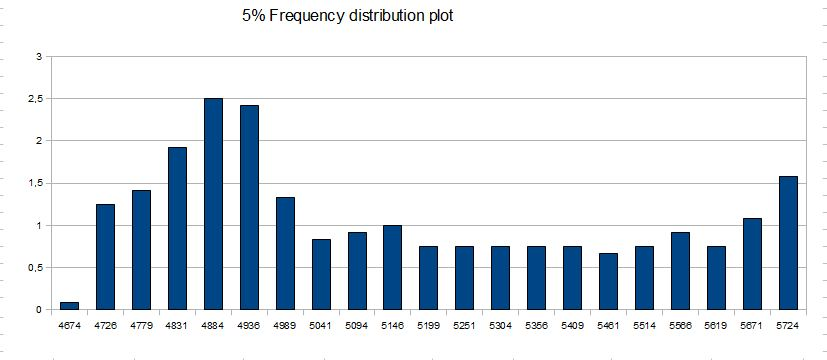
\includegraphics[width=1.0\textwidth]{Images/TF_timer.jpg}
 \caption{Eksempel på omgjøring til timer}
\end{figure}


Vi gjorde om antall logginger til timer, slik at man lettere ser hvor mange timer det tok for hver ca.  50. insert-spørring. Da er det også veldig lett å telle seg frem til hvor i døgnet man er.\\

- Forklaring av tabellene.\\
Vi ser i tabellene at verdien går mellom 4000 og 6000. Percentilen vil i dette tilfelle vise i prosent hvor mange sjekker som har foregått fra og med Rad1 til og med den enkelte raden. Tallet blir basert på det totale antallet sjekker. F.eks:
\begin{itemize}
\item Rad 2: 4779 inserts på 32 sjekker - 11,87 - i 10\% percentile
\item Rad 3: 4884 inserts på 53 sjekker - 30,94 - i 10\% percentile
\item Rad 4: 4989 inserts på 45 sjekker - 47,12 - i 10\% percentile
\end{itemize}

Ut fra disse opplysningene kan vi se at Rad 3 hadde mange flere sjekker enn Rad 2, mens antall inserts er det samme. 10\% percentilen på Rad 3 er 30,94, og dette betyr at rundt 30\% av alle sjekkene skjedde mellom Rad1 og Rad3. Det betyr også at det ble brukt 30\% av hele tidsperioden på mellom Rad1 og Rad3. Dersom vi ser på Rad3 spesifikt, ser vi at denne er 19,07 mer i percentile enn i Rad2. Denne verdien viser at rundt 20\% av alle sjekkene skjedde mellom Rad2 og Rad3, som også betyr at det var veldig lite aktivitet i det tidsrommet frem til neste rad.

\begin{figure}[h!]
 \centering
  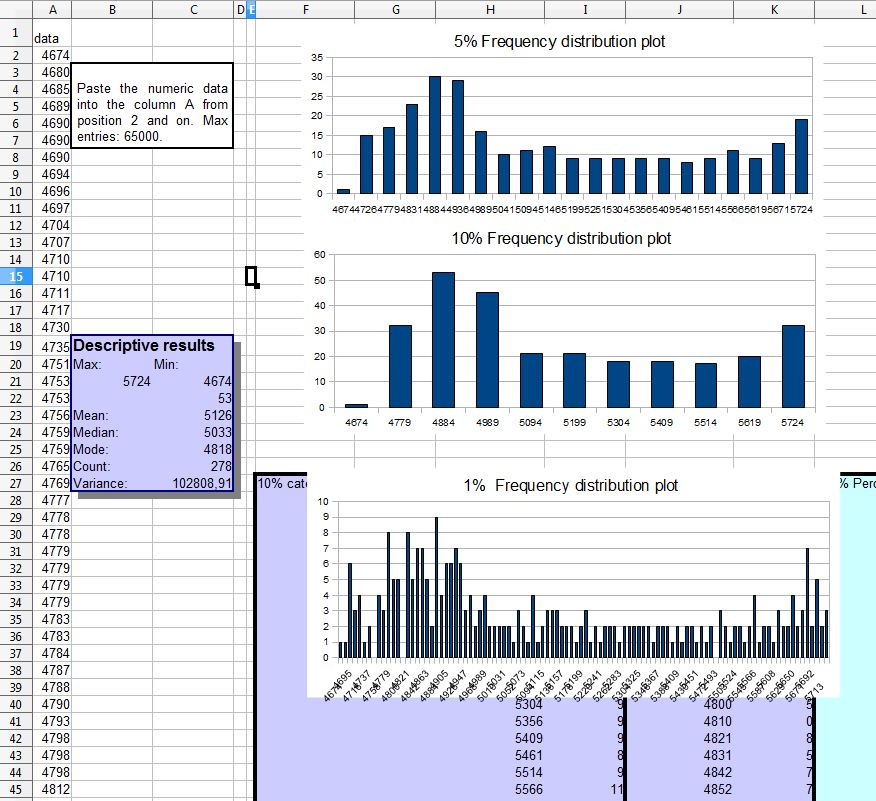
\includegraphics[width=0.8\textwidth]{Images/Insert_i_TF_calc.jpg}
 \caption{Screenshot av dataene}
\end{figure}

\subsection{Oppgave 3}
\subsubsection*{3.1}
Fra mandag til mandag to uker etter så serveren ut til å bruke 5.8 Mb mer trafikk. Om vi tar 100Mb delt på 5.8Mb får vi vite at det vil ta 17.24 to-ukersperioder fær nettet er fylt opp med den samme stigningen man har nå. Ganger man det med to får vi 34.48 uker.

\subsubsection*{3.2}
Forrige oppgave hadde en 100Mb link og fikk 34.5 uker. Dersom vi har en 1Gb link som er 10 ganger så stor, kan vi gange resultatet i forrige oppgave med 10 for å få svaret. Dvs 344,8 uker, eller 6 år og 31 uker.

\subsubsection*{3.3}
Dersom vi følger samme oppsett som 3.1 og 3.2 får vi 3448 uker, eller 66 år og 15 uker.

\subsubsection*{3.4}
Vi antar at disse resultatene er sannsynlige. Det at man sprenger kapasiteten på kun 34.48 uker er noe man må gjøre noe med, dette er alt for nært til at man kan vente med å se hva som skjer.. Hva som skjer seks år eller 66 år frem i tid er ikke den største bekymringa i dag. Da vil all teknologi og nettstandarder være et helt annet sted enn i dag. Noe man derimot bør ha i tankene er hvordan behovet ser ut til å bli om tre år, slik at man har en plan for det. Det at stigningen er linjær gjør at det er lettere å tilpasse seg behovet for nett, fremfor om trafikken gikk i veldige store svingninger uten noe mønster.\\

Man kan se på hvor store f.eks. profilbilder som hele tiden blir vist er. Disse bør ta så liten plass de kan og enda være av grei kvalitet i størrelsen de blir vist i.\\

For å rette problemet kan vi:
\begin{itemize}
\item overvåke
\item skaffe større link
\item teste ytelse (aktiv og passiv)
\end{itemize}

Ytelse foregår ikke bare på applikasjonsnivå, men på veldig mange nivåer helt ned til diskplatene, og alle disse nivåene kan testes på et vis. Nøkkelen til god ytelsesanalyse er å få riktig oversikt over systemets oppførsel. Det er viktig å overvåke om systemet er raskt nok til enhver tid.\\

Der finnes to måter å teste ytelse på: aktiv og passiv. Ved aktiv ytelse går en inn og presser ytelsen til det maksimale. Her finner vi gjerne ekstremverdier som vi ofte ikke ser i vanlig bruk. Passive tester samler derimot reelle data fra vanlig bruk. Der finnes et filsystem, Bonnie++, som bruker systemkall og måler hvor lang tid de tok, som vi kan bruke. Der finnes også andre metoder.


%\clearpage
%\addcontentsline{toc}{section}{Referanser} %Add this section to content table
%\bibliographystyle{unsrt} % change for dcu, or something else entirely? unsrt is nice !- referanser
%\bibliography{Referanser}

%\addcontentsline{toc}{section}{Vedlegg} %Add this section to content table
%\section*{Vedlegg}

\end{document}
